\chapter{Theory}
Before we started our project, we did quite alot of prestudy, covering which technology was available, to determine which fit our project best. This chapter will contain a summary of the different technologies, and also some theory behind the reasoning for having multiple ground stations listen to our satelite.
\section{Communicating with the satelitte}

\begin{figure}
	\begin{center}
		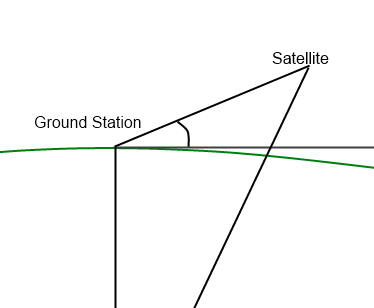
\includegraphics[width=0.7\textwidth]{Figures/groundstation_satelitte_geometry}
	\end{center}
\caption[Ground station satellite geometry]{Illustration of geometry between a ground station and a satelitte}
\label{fig:gs_s_geom}
\end{figure}

A ground station can only communicate with a satelitte when it has a certain elevation. This elevation can differ from case to case depending on atmospheric effects, frequency and more. 
In the following we assume that the minimum elevation is 25 degrees, maximum elevation is 90 degrees and no constraints on the azimuth angle.  For a illustration see Fig. \ref{fig:gs_s_geom}.


The result of this is that the ground station can communicate with the satelitte whenever the ground track is inside a rough circle centered on the ground station, see Fig. \ref{fig:ntnu_range} for the estimated "range" of the ground station at Gløshaugen operating with these constraints.

This ground station will, on average, be able to communicate with the satellite xx seconds per day. That means that we will be able to download

\begin{equation}
D=2.4 kbps \cdot xx s = yy kb
\end{equation} 

\begin{figure}
	\begin{center}
		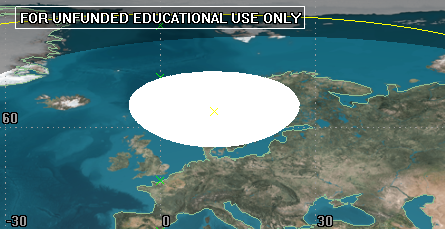
\includegraphics[width=0.8\textwidth]{Figures/ntnu_footprint}
	\end{center}
\caption[ntnu footprint]{NTNU ground station range}
\label{fig:ntnu_range}
\end{figure}
\section{Network technology for ground stations}
When we decided to work on a network of ground stations, we first looked into four different ground station network technologies. We first hoped to work on a BlueBox, but this would require support from Aalborg that we couldn't get, as they were busy with a satelite launch of their own. Because of this, we decided to look into Carpcomm, that seemed more complete and doable than connecting to PYXIS with a BlueBox.
\subsection{Pico}


\subsection{Genso}
information about Genso
\subsection{Carpcomm Space Network}
Carpcomm is a private company that delivers a plug and play ground station \cite{carpcomm-gs1} that costs \$700. The software for the ground station is open source and is provided pre.compiled for x86 and arm debian.
It is compatible with the Carpcomm Space Network \cite{carpcomm-sn}. 
The advantage of using this solution is that the network is actually functioning, though there are few other operational ground stations.
%\cite{carpcomm-gs1}
%\cite{carpcomm-sn}
\subsection{PYXIS}
The BlueBox is part of a distributed ground station network called PYXIS, developed primarily for the AAUSAT3 by Aalborg University (2013 \cite{aausat3}). The PYXIS goal is to offer a robust and effective ground station network for satellite developers, and one of the key factors is that everyone is free to setup a ground station using the open source BlueBox hardware. 

The PYXIS concept includes a backend server, BlueBox hardware and a Ground Station Server (GSS). The backend server runs an individual instance for each satellite utilizing the BlueBox, and is operated by the persons responsible for the ground station. 

The BlueBox itself is hardware to recieve and transmit signlas from the satellites.

Control of the BlueBox and ground station mechanics is handled by the GSS, and both the BlueBox and the GSS is operated by the responsible for the Ground station. 

Both the backend server and the GSS is already in place at each ground station, and to join the PYXIS network we would only have to make a BlueBox, and test that it works.

\section{Raspberry pi}
Raspberry Pi is a small computer, with everything gathered in one board. In our project we will be using the B model, revision 2, which have a 700MHz ARM CPU, 512MB of RAM and a SC-card reader, in addition to the leads to connect to different devices, for  the full overview, see figure \ref{fig:raspberrypihighlevel}. The recommended operating system is Raspbian, a linux distribution based on Debian. 

The Raspberry pi was originally intended to help teach programming, but it can also perform many of the standard computer tasks, and it can be connected to a monitor or tv using an HDMI lead. In our project we hope to be able to use a Raspberry pi to run the software required to control the ground stations. The software provided by the Carpcomm project has Raspbian as one of its supported platforms, so we hope this will work well.

\begin{figure}
	\begin{center}
		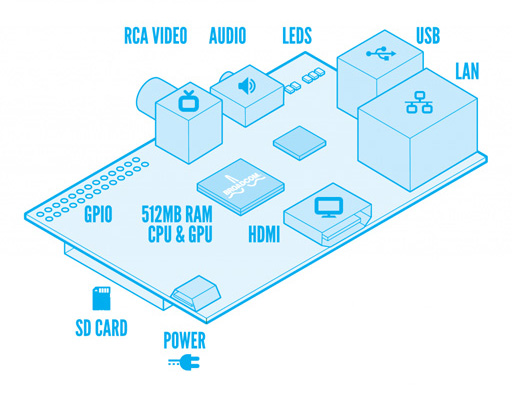
\includegraphics[width=0.7\textwidth]{Figures/raspberrypi_modelb_hl.jpg}
	\end{center}
	\caption[Raspberry pi highlevel]{A highlevel schemantic of the Raspberry pi, model B rev 2}
	\label{fig:raspberrypihighlevel}
\end{figure}

To control the movement of the antennas, an serial port is needed. Raspberry Pi has an serial port included in its gpio (general purpose input/output) connector. This serial port uses ttl-standard for its voltage levels, this is 0/3.3V while RS232 which is the standard used in computers uses (3V-15V)/-(3V-15V). Because of this an converter is needed. We chose to make an custom circuit board using the MAX3232 RS232 line driver. The circuit board is designed to be mounted on the gpio connector, because of small space in the case for the Raspberry Pi, the output is connected with cable to the external connector.

\begin{figure}
	\begin{center}
		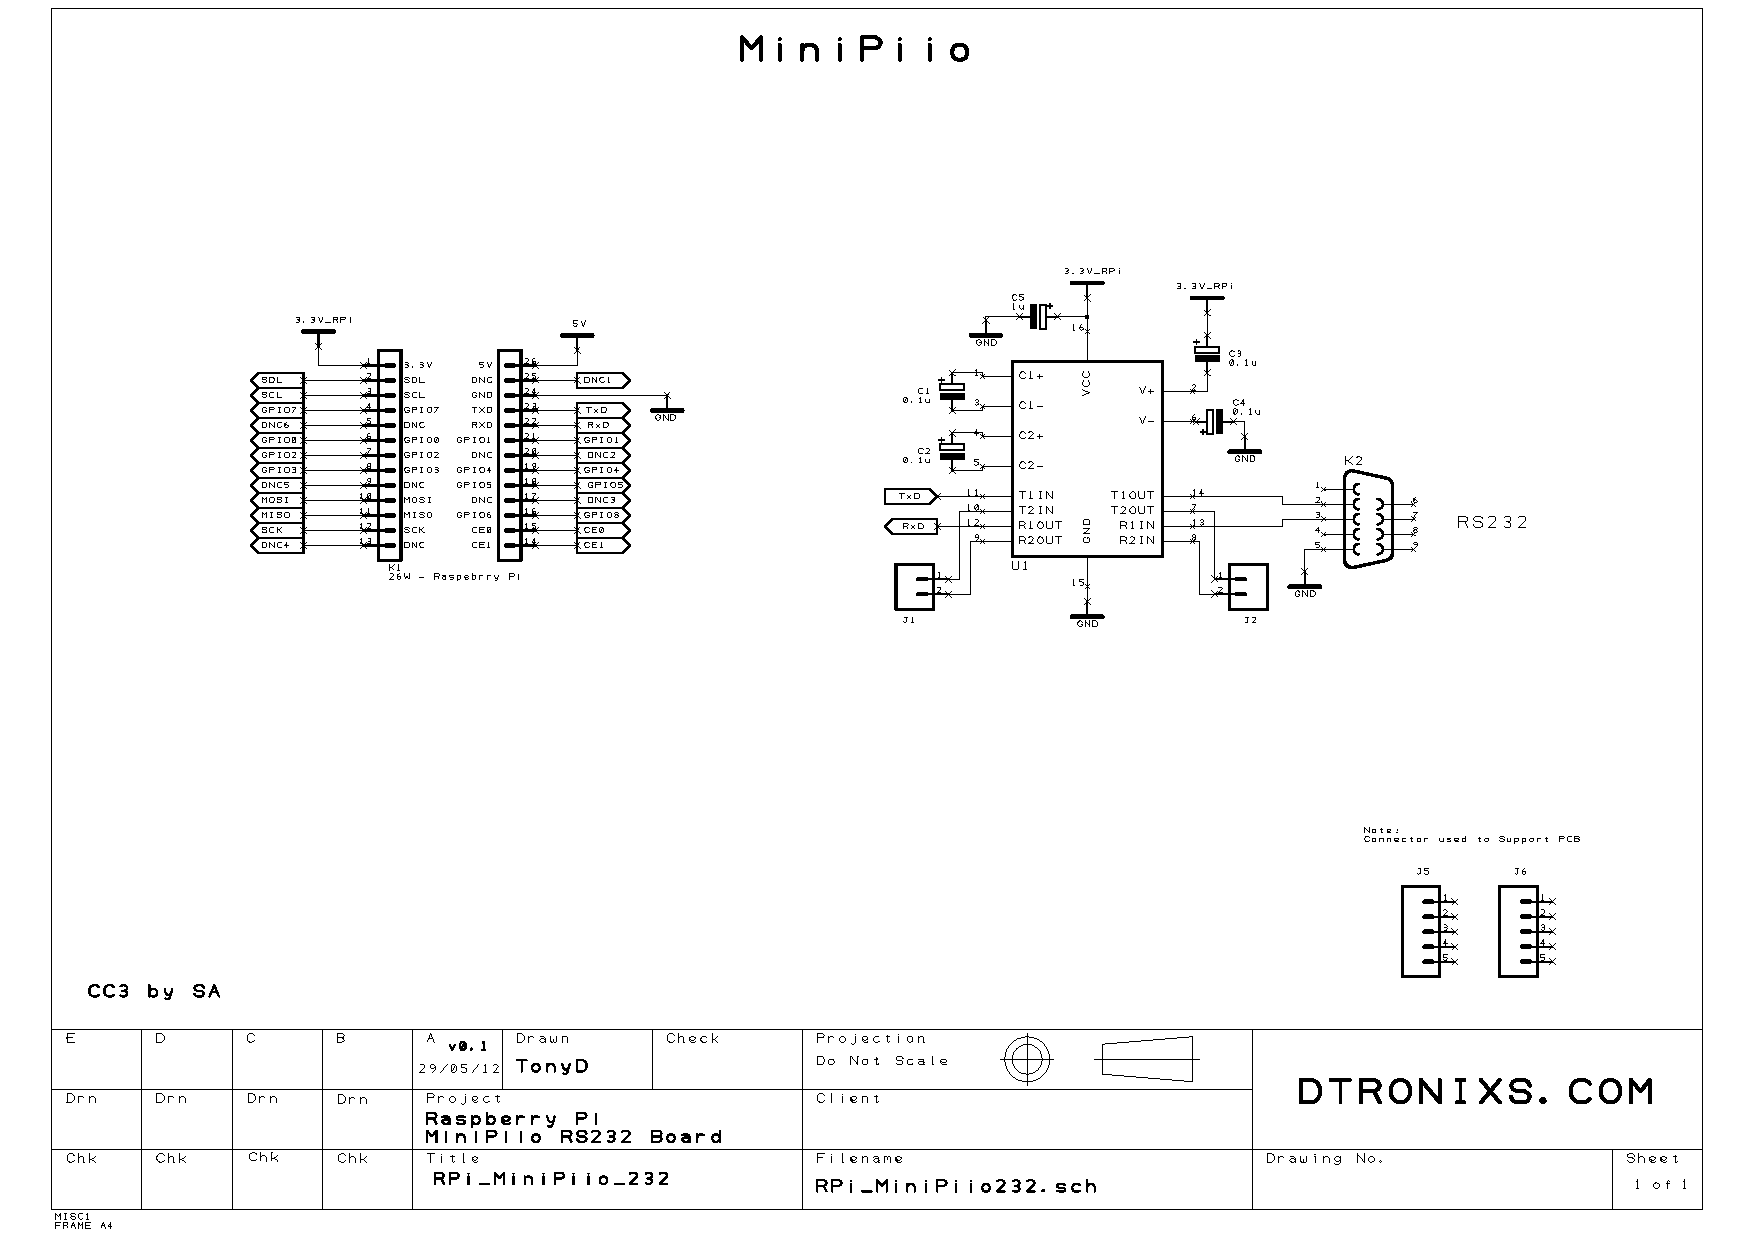
\includegraphics[width=0.7\textwidth, trim=400 250 100 100, clip=true]{../Schematics/UART-to-RS232.pdf}
	\end{center}
	\caption{Schematics for the RS232-converter}
	\label{fig:UART-RS232}
\end{figure}
\input{Theory/SunPower}

